%% Porocilo iz vaj pri reologiji
%% Junij 2015
%% Ivan Pribec, Jasmina Sedmak, Filip Strniša

\documentclass{article}

\usepackage{color}
\usepackage{epsfig,graphics}
\usepackage{amsmath}

\usepackage[utf8]{inputenc}
\usepackage[protrusion=true,
            expansion=true
           ]{microtype}

\usepackage[slovene]{babel}
\usepackage{graphicx} 
\usepackage{caption}          % Needed for including graphics.
\usepackage{url}                % Facility for activating URLs.

\usepackage[a4paper,margin=2.4cm]{geometry}

\usepackage{tabularx}
\newcolumntype{Y}{>{\centering\arraybackslash}X}

\usepackage{subcaption}
\usepackage{wrapfig}
\usepackage{sidecap}
\usepackage{breakurl}
\usepackage{booktabs}
\usepackage{float}
\setlength{\heavyrulewidth}{1.1pt}
\setlength{\abovetopsep}{1pt}

\renewcommand{\refname}{Literatura} 

%%%%%%%%%%%%%%%%%%%%%%%%%%%%%%%%%%%%%%%%%%%%%%%%%%%%%%%%%%%%%%%%%%%%%%
%% Start of the document.
%%%%%%%%%%%%%%%%%%%%%%%%%%%%%%%%%%%%%%%%%%%%%%%%%%%%%%%%%%%%%%%%%%%%%%

\begin{document}

\author{Ivan Pribec, Jasmina Sedmak, Filip Strniša\\
Fakulteta za kemijo in kemijsko tehnologijo, Univerza v Ljubljani}
\date{Ljubljana, 09.07.2015}
\title{Poročilo iz vaj pri predmetu \textit{Reologija kompleksnih tekočin}\\
Reološke lastnosti raztopin ksantana in gelana}
\maketitle


\section{Namen vaje}
Cilj tokratnih vaj iz reologije je bila seznanitev z uporabo rotacijskega viskozimetra z nastavljivo strižno napetostjo in spoznavanje različnih merilnih tehnik pri nedestruktivnih in destruktivnih strižnih pogojih. Poseben poudarek je bil na merilnih tehnikah za viskoelastične tekočine (oscilatorni testi in testi lezenja in obnove). Pridobljene rezultate smo tudi interpretirali s pomočjo različnih reoloških modelov in risanjem reoloških grafov. Testirane snovi so bile vodne raztopine polisaharidov gelana in ksantana.

\section{Teoretične osnove in metode dela}

Pojem \textbf{gel} se uporablja za opisovanje želatini podobne, bolj ali manj rigidne snovi, ki se tvori s tem, ko se koloidni delčki med seboj povežejo v tridimenzionalno mrežo ali pa pri premreženju polimernih molekul. Čeprav lahko večino mase gela predstavlja tekočina (npr. voda) je premreženje tisto, ki daje gelu svoje trdno strukturo. Veliko gelov izkazuje tiksotropijo, saj se ob agitaciji njihova struktura podre in lahko stečejo. Prav tako izkazujejo mejno napetost in viskoelastične lasnosti.
Na vaji smo za pripravo vzorcev uporabila dva polisaharida:
\begin{itemize}
\item KSANTAN je naravni polisaharid, ki nastane pri fermentaciji sladkorjev s z bakterijo \textit{Xanthomonas campestris}. Uporablja se ga kot regulator viskoznosti, gostilo, gelirno sredsvo in stabilizator emulzij v prehranski (E415; pudingi, solatne polivke, sladoled in peka kruha) in kozmetični industriji (kreme, losjoni, zobna pasta).
 \item GELLAN je anionski polisaharid, ki ga proizvajajo bakterije \textit{Sphingomonas elodea}. Uporablja se ga kot alternativno gelirno sredstvo agarju v mikrobiologiji in pri gojenju rastlinskih celičnih kultur. Uporabo pa ima tudi v prehranski (E418), kozmetični in farmacevtski industriji kot gostilo, emulgator, stabilizator in gelirno sredstvo.
\end{itemize}

Iz že pripravljenega gela dane koncentracije polisaharida smo vzeli izračunano količino in jo raztopili v vodi, segreli do vrenja in prekuhali za 10 minut. Tako smo pripravili 0,5, 0,7 in 1,0 \% raztopine gelana in 1,0 \% raztopino ksantana. Kljub nizkim koncentracijam imajo take raztopine šibkogelski značaj.

Najpopularnejši instrument za reološko karakterizacijo snovi je zagotovo \textbf{rotacijski viskozimeter} kot je prikazan na sliki \ref{fig:viskozimeter}. Deluje na principu merjenja navora, ki je potreben, da vrtimo senzorski sistem v stiku s tekočino. Na podlagi vrtilne hitrosti in geometrije senzorskega sistema lahko izračunamo viskoznost tekočine. Takemu reometru pravimo tudi reometer z nastavljivo strižno hitrostjo. Modernejši tip reometra, je rotacijski viskozimeter z nastavljivo strižno deformacijo. V takem reometru je nastavljena vrednost navora, odpor vzorca proti nastavljeni strižni napetosti pa povzroči odmik rotorja. Hitrost rotorja in pozicijo se izmeri z digitalnim optičnim kodirnikom. Sistem mora biti zračno uležajen. Reometer z nastavljivo strižno napetostjo omogoča izvedbo zahtevnejših merilnih tehnik kot so testi lezenja in obnove ter oscilatorni testi.

\begin{figure}
   \centering
   \begin{subfigure}[b]{0.3\textwidth}
       \includegraphics[width=\textwidth]{rheometer2.jpg}
   \end{subfigure}
   \qquad %add desired spacing between images, e. g. ~, \quad, \qquad, \hfill etc. 
     %(or a blank line to force the subfigure onto a new line)
   \begin{subfigure}[b]{0.4\textwidth}
       \includegraphics[width=\textwidth]{plosca_plosca.jpg}
   \end{subfigure}
   
   \caption{Rotacijski viskozimeter in senzorski sistem dveh vzporednih plošč podoben tistemu, ki smo ga uporabili med izvedbo vaje. Vir: \burl{http://www.usm.flaneyassociates.com/ResearchFacilities/Rheology.htm}}
   \label{fig:viskozimeter}
\end{figure}

Za reološko karakterizacijo snovi se na rotacijskem viskozimetru poslužujemo različnih merilnih tehnik, pri katerih vzorce izpostavimo statičnim ali dinamičnim strižnim pogojem in sledimo obnašanju materiala preko količin kot so navidezna viskoznost $\eta$, strižna deformacija $\gamma$, strižna hitrost $\dot{\gamma}$, strižna napetost $\tau$, modul akumulacije energije $G^{'}$, modul energetskih izgub $G^{''}$, faktor dušenja $\delta$, kompleksni modul $G^*$ in voljnost $J$. Med vajo smo izmerili naslednje odvisnosti oz. napravili napisane teste:
\begin{enumerate}
\item Tokovna odvisnost (trikotna metoda)
\item Temperaturna odvisnost
\item Amplitudna odvisnost (oscilatorni test)
\item Frekvenčna odvisnost (oscilatorni test)
\item Test lezenja in obnove
\item Ponavljajoči test lezenja in obnove
\end{enumerate}
Več o posamezni metodi in same pogoje meritev smo podali v poglavju \ref{pog:mer} - Meritve in rezultati.

Po izvedbi reoloških meritev se pogosto soočamo s problemom, da moramo izmerjenim eksperimentalnim točkam poiskati modelno funkcijo, ki te točke najbolje opiše. S pomočjo modelnih funkcij nato lažje primerjamo vpliv preučevanih spremenljivk (npr. koncentracije, temperature) na dano snov. Reološke modelne funkcije so v večini nelinearne, kar zahteva prav posebno skrb. Imamo torej \textbf{optimizacijski problem}, ki ga rešujemo s pomočjo minimizacije vsote kvadratov razlik med izmerjenimi in funkcijskimi vrednostmi
\begin{equation}
S = \sum\limits^N_i \big(y^\mathrm{meritev}_i-y^\mathrm{model}_i(x^\mathrm{meritev}_i,\mathrm{\textbf{v}})\big)^2
\end{equation}
kjer par ($x^\mathrm{meritev}_i,y^\mathrm{meritev}_i$) predstavlja izmerjene eksperimentalne vrednosti, $y^\mathrm{model}_i(x^\mathrm{meritev}_i,\mathrm{\textbf{v}})$ izračunane vrednosti po funkciji izbranega modela, $\mathrm{\textbf{v}}$ je vektor parametrov, ki nastopajo v modelni funkciji in $N$ število eksperimentalnih točk. Reševanja takega problema se lotimo numerično s pomočjo izdelanih programov kot sta Excel (orodje \textit{Solver}) in Matlab (funkcija \texttt{lsqnonlin}), ali pa izdelamo svoj program na osnovi jezika Python in različnih namenskih knjižnic (\texttt{scipy.optimize}, \texttt{lmfit}).

\section{Meritve in rezultati} \label{pog:mer}

Študenti smo bili pri izvedbi vaj razdeljeni v 2. skupini. V nadaljevanju bodo predstavljeni rezultati obeh skupin, saj smo tako dobili bolj celovito sliko (1. skupina ni opravila nekaterih testov in obratno). V splošnem nas je zanimalo obnašanje raztopin gelana pri različnih koncentracijah (0,5, 0,7 in 1,0 \%) in obnašanje ksantana pri temperaturah 20 in 30 $^\circ$C. Kljub obravnavi podatkov obeh skupin smo nekaj podatkov ob prenosu na računalnik izgubili.

\subsection{Tokovna odvisnost}

Določitev tokovne odvisnosti je potekala na ta način, da smo vzorce nanesli med plošče reometra in jih izpostavili strižnim hitrostim v območju med 0,01 in 100 s$^-1$ (strižno hitrost smo spreminjali v obe smeri). Viskozimeter je tako beležil odvisnost strižne napetosti od strižne hitrosti in tudi izračunal navidezno viskoznost pri danih strižnih pogojih po enačbi \ref{eq:visc}. Za lažjo primerjavo vzorcev je smiselno, da rezultate opišemo z modelno funkcijo in primerjamo parametre izbranih funkcij. Nato smo preverili, kako rezultati pašejo v razširjen Cassonov (enačba (\ref{eq:powerm})) in Crossov model (enačba (\ref{eq:Crossm})).

\begin{equation} \label{eq:visc}
\eta = \frac{\tau}{\dot{\gamma}} = f(\tau)
\end{equation}

\begin{equation} \label{eq:powerm}
\tau^n = {\tau_0}^n + \Big(\eta_\infty\dot{\gamma}\Big)^n
\end{equation}

\begin{equation} \label{eq:Crossm}
\frac{\eta - \eta_{\infty}}{\eta_0 - \eta_{\infty}} = \frac{1}{1 + \Big(K_1\dot{\gamma}\Big)^m}
\end{equation}

\subsubsection{Crossov model}

\begin{figure}[H]
	\centering
	\begin{subfigure}[b]{0.45\linewidth}
	       \includegraphics[width=\linewidth]{cross_ksan1.eps}
	   \end{subfigure}
	   ~
	   \begin{subfigure}[b]{0.45\linewidth}
	       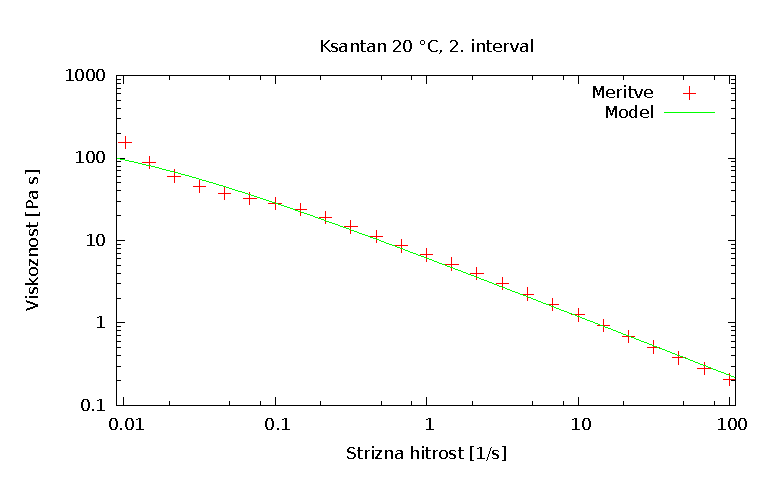
\includegraphics[width=\linewidth]{cross_ksan2.eps}
	   \end{subfigure}
	\caption{Meritve za 1 \% Ksantan pri 20 $^\circ$C. 1. interval: $K_1 = 138,5 s; m = 0,858; \eta_0 = 731,4 Pa s; \eta_\infty = 0,0345 Pa s$. 2. interval: $K_1 = 138,5 s; m = 0,717; \eta_0 = 215,8 Pa s; \eta_\infty = 0 Pa s$.}
	\label{fig:cross_xan1}
\end{figure}

\begin{figure}[H]
	\centering
	\begin{subfigure}[b]{0.45\textwidth}
	       \includegraphics[width=\textwidth]{cross_ksan3.eps}
	   \end{subfigure}
	   ~
	   \begin{subfigure}[b]{0.45\textwidth}
	       \includegraphics[width=\textwidth]{cross_ksan4.eps}
	   \end{subfigure}
	\caption{Meritve za 1 \% Ksantan pri 30 $^\circ$C. 1. interval: $K_1 = 116,9 s; m = 0,793; \eta_0 = 348,5 Pa s; \eta_\infty = 0 Pa s$. 2. interval: $K_1 = 96,1 s; m = 0,760; \eta_0 = 231,6 Pa s; \eta_\infty = 0 Pa s$.}
	\label{fig:cross_xan2}
\end{figure}

\begin{figure}[H]
	\centering
	\begin{subfigure}[b]{0.45\textwidth}
	       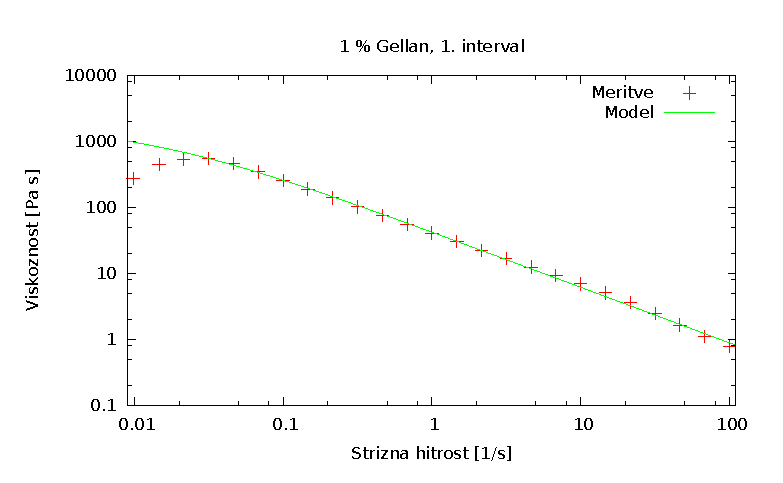
\includegraphics[width=\textwidth]{cross_gel1.eps}
	   \end{subfigure}
	   ~
	   \begin{subfigure}[b]{0.45\textwidth}
	       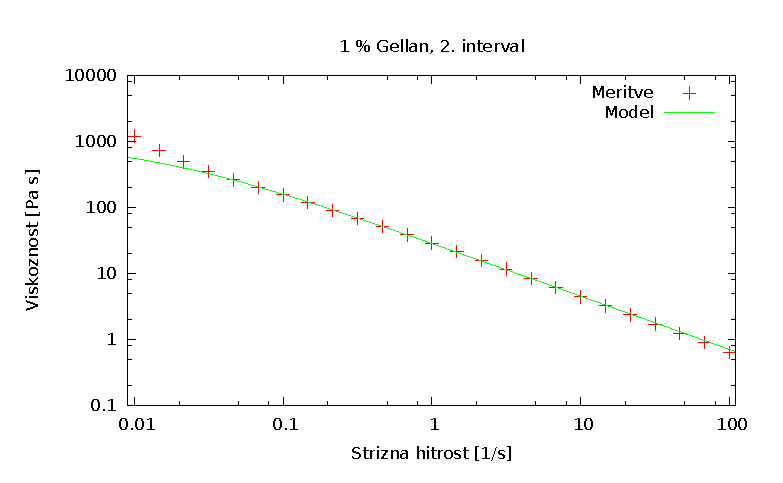
\includegraphics[width=\textwidth]{cross_gel2.eps}
	   \end{subfigure}
	\caption{Meritve za 1 \% Gellan pri 20 $^\circ$C. 1. interval: $K_1 = 83,54 s; m = 0,844; \eta_0 = 1814 Pa s; \eta_\infty = 0 Pa s$. 2. interval: $K_1 = 80,87 s; m = 0,809; \eta_0 = 1022 Pa s; \eta_\infty = 0 Pa s$.}
	\label{fig:cross_gel1}
\end{figure}

\begin{figure}[H]
	\centering
	\begin{subfigure}[b]{0.45\textwidth}
	       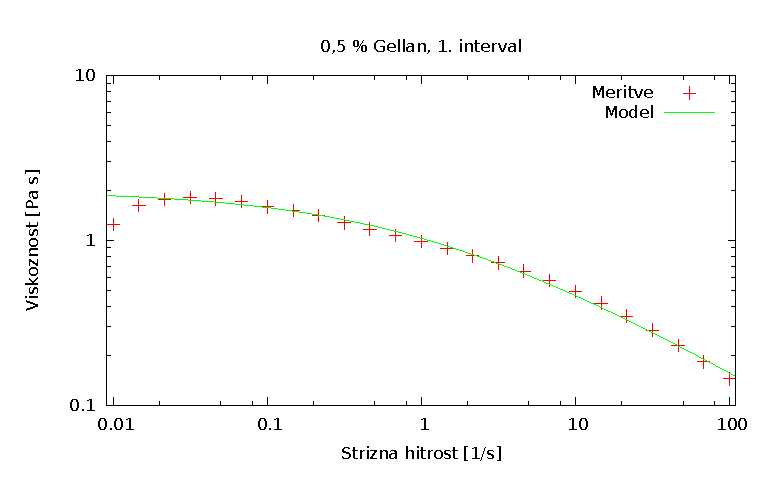
\includegraphics[width=\textwidth]{cross_gel3.eps}
	   \end{subfigure}
	   ~
	   \begin{subfigure}[b]{0.45\textwidth}
	       \includegraphics[width=\textwidth]{cross_gel4.eps}
	   \end{subfigure}
	\caption{Meritve za 0,5 \% Gellan pri 20 $^\circ$C. 1. interval: $K_1 = 0,902 s; m = 0,548; \eta_0 = 2,007 Pa s; \eta_\infty = 0 Pa s$. 2. interval: $K_1 = 0,212 s; m = 0,662; \eta_0 = 1,277 Pa s; \eta_\infty = 0 Pa s$.}
	\label{fig:cross_gel2}
\end{figure}

\subsubsection{Razširjen Cassonov model}

\begin{figure}[H]
	\centering
	\begin{subfigure}[b]{0.45\textwidth}
	       \includegraphics[width=\textwidth]{tok_ksan1.eps}
	   \end{subfigure}
	   ~
	   \begin{subfigure}[b]{0.45\textwidth}
	       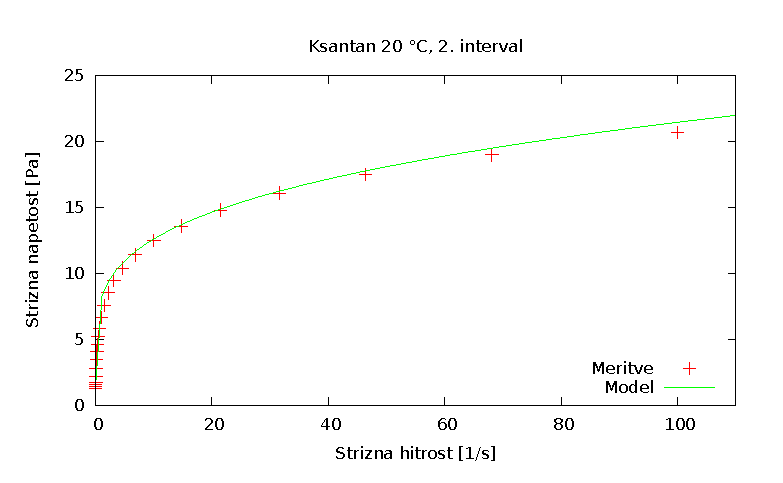
\includegraphics[width=\textwidth]{tok_ksan2.eps}
	   \end{subfigure}
	\caption{Meritve za 1 \% Ksantan pri 20 $^\circ$C. 1. interval: $n = 0,107; \tau_0 = 2,414 Pa; \eta_\infty = 1,63*10^{-7} Pa s$. 2. interval: $n = 0,108; \tau_0 = 1,422 Pa; \eta_\infty = 6,15*10^{-7} Pa s$.}
	\label{fig:tok_ksan1}
\end{figure}

\begin{figure}[H]
	\centering
	\begin{subfigure}[b]{0.45\textwidth}
	       \includegraphics[width=\textwidth]{tok_ksan3.eps}
	   \end{subfigure}
	   ~
	   \begin{subfigure}[b]{0.45\textwidth}
	       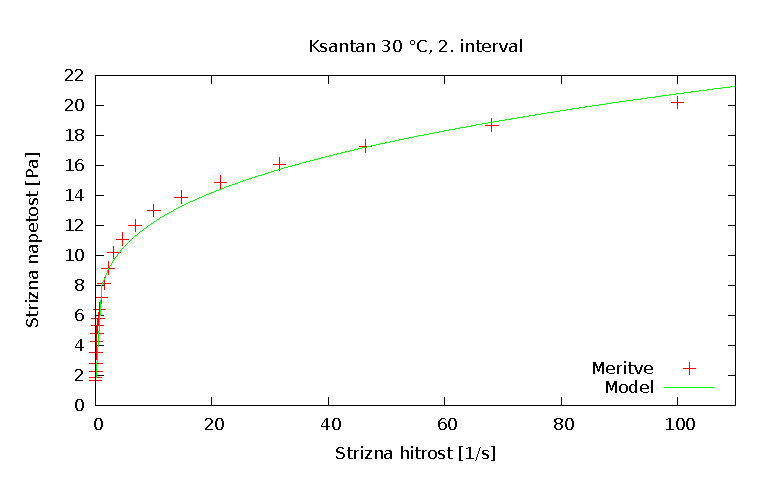
\includegraphics[width=\textwidth]{tok_ksan4.eps}
	   \end{subfigure}
	\caption{Meritve za 1 \% Ksantan pri 30 $^\circ$C. 1. interval: $n = 0,107; \tau_0 = 1,397 Pa; \eta_\infty = 5,26*10^{-7} Pa s$. 2. interval: $n = 0,107; \tau_0 = 1,351 Pa; \eta_\infty = 5,26*10^{-7} Pa s$.}
	\label{fig:tok_ksan2}
\end{figure}

\begin{figure}[H]
	\centering
	\begin{subfigure}[b]{0.45\textwidth}
	       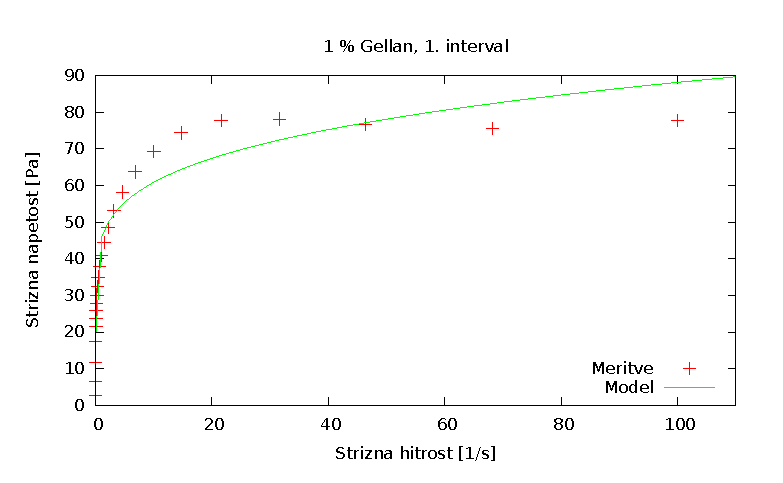
\includegraphics[width=\textwidth]{tok_gel1.eps}
	   \end{subfigure}
	   ~
	   \begin{subfigure}[b]{0.45\textwidth}
	       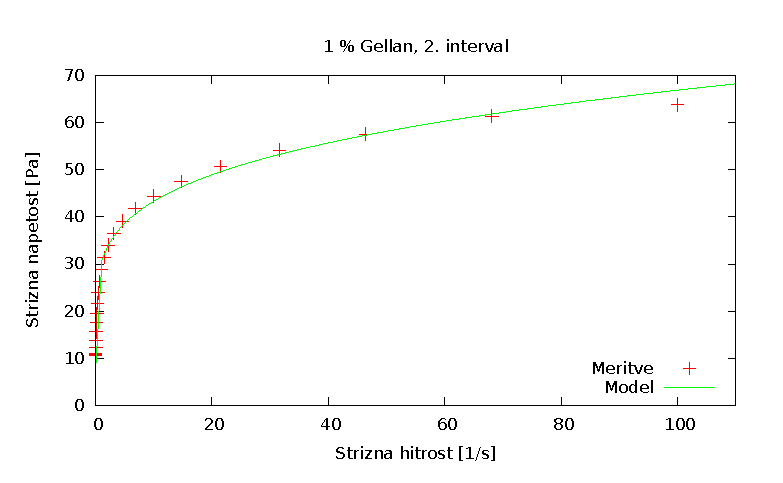
\includegraphics[width=\textwidth]{tok_gel2.eps}
	   \end{subfigure}
	\caption{Meritve za 1 \% Gellan pri 20 $^\circ$C. 1. interval: $n = 0,125; \tau_0 = 17,84 Pa; \eta_\infty = 9,81*10^{-7} Pa s$. 2. interval: $n = 0,105; \tau_0 = 7,270 Pa; \eta_\infty = 2,06*10^{-7} Pa s$.}
	\label{fig:tok_gel1}
\end{figure}

\begin{figure}[H]
	\centering
	\begin{subfigure}[b]{0.45\textwidth}
	       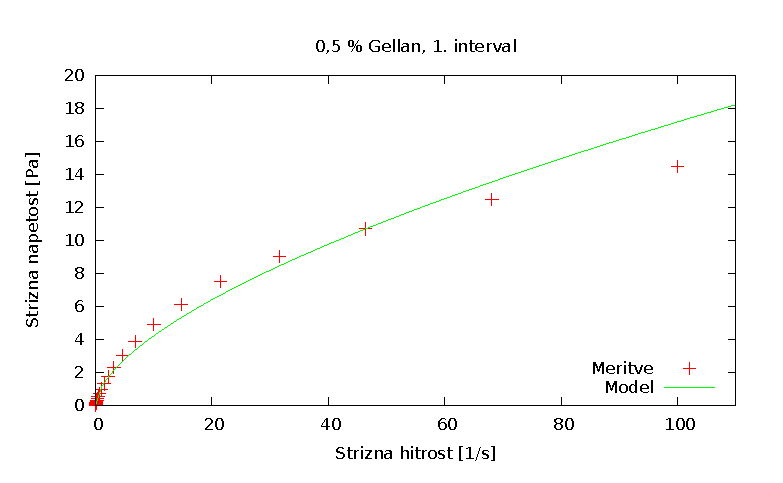
\includegraphics[width=\textwidth]{tok_gel3.eps}
	   \end{subfigure}
	   ~
	   \begin{subfigure}[b]{0.45\textwidth}
	       \includegraphics[width=\textwidth]{tok_gel4.eps}
	   \end{subfigure}
	\caption{Meritve za 0,5 \% Gellan pri 20 $^\circ$C. 1. interval: $n = 0,0396; \tau_0 = 4,0*10^{-10} Pa; \eta_\infty = 1,03*10^{-6} Pa s$. 2. interval: $n = 0,0396; \tau_0 = 3,97*10^{-10} Pa; \eta_\infty = 1,05*10^{-6} Pa s$.}
	\label{fig:tok_gel2}
\end{figure}

\subsection{Temperaturna odvisnost}

Na reometru smo merili viskoznost 1 \% Gellana na temperaturnem intervalu 15 - 50 $^\circ$C pri konstantni strižni hitrosti 50 $s^{-1}$. Temperaturo smo spreminjali v obe smeri.
Na grafu \ref{fig:temp} je razvidno, da viskoznost pada z naraščanjem temperature. V območju med 29 in 34 $^\circ$C je viskoznost padla za red velikosti. Podatki za gelan kažejo, da ima ta v tem območju gelirno točko. Pri segrevanju se torej struktura podre, pri ohlajanju pa se pri tej temperaturi gelan ponovno zamreži in viskoznost naraste. Nižja viskoznost ob koncu ohlajevanja je verjetno posledica še ne popolnoma obnovljene notranje stukture.

\begin{figure}[H]
  \centering
  \includegraphics[width=0.8\linewidth]{temperature.png}
  \caption{Viskoznost raztopine gelana v odvisnosti od temperature $T$. Zgornja krivulja je bila dobljena med segrevanjem, spodnja pa med ohlajanjem vzorca.}
  \label{fig:temp}
\end{figure}


\subsection{Amplitudna odvisnost}

Območje linearnega viskoelastičnega odziva (LVO) smo določali z amplitudnim testom, kjer povečujemo amplitudo strižne deformacije pri konstantni frekvenci oscilacije. Kritično vrednost $\gamma_\mathrm{krit}$ smo določali na ta način, da smo eksperimentalnim podatkom prilagodili naslednjo funkcijo za kompleksni strižni modul ($G^* = \sqrt{(G^{'})^2 + (G^{''})^2}$):
\begin{equation} \label{eq:ampl}
G^* = G^*_0\frac{1+b\gamma^n}{1+a\gamma^n}
\end{equation}
in izračunali vrednost $\gamma$, kjer doseže $G^*$ 3 \% odstopanje od začetne vrednosti $G^*_0$:
\begin{equation}
\gamma_\mathrm{krit}=\Bigg( \frac{1-\frac{G^*}{G^*_0}}{\frac{G^*}{G^*_0}b-a} \Bigg)^{\frac{1}{n}} = \Bigg( \frac{0,03}{0,97b-a} \Bigg)^{\frac{1}{n}} .
\end{equation}

Meritve za obe skupini sta prikazani na slikah \ref{fig:ampl1} in \ref{fig:ampl2}, parametri enačbe \ref{eq:ampl} in kritične vrednosti deformacije pa so zbrane v tabelah \ref{tab:ampl1} in \ref{tab:ampl2}. Na vzorcih gelana je razvidno, da z večanjem koncentracija polisaharida, s tem ko postane material bolj ``trden'', se območje LVO oži. V primeru ksantana pri dvigu temperature z 20 na 30 $^\circ$C je opazen majhen vpliv (pri višji temperaturi je bolj ``tekoč''),

\begin{figure}
  \centering
  \includegraphics[width=\linewidth]{S1ampl.png}
  \caption{Določitev območja linearnega viskoelastičnega odziva raztopinam ksantana in gelana s šibkogelskim značajem. Prikazane so meritve 1. skupine. Polna črta predstavlja modelno enačbo \ref{eq:ampl}, vertikalna črta pa kritično vrednost strižne deformacije.}
  \label{fig:ampl1}
\end{figure}

\renewcommand{\arraystretch}{1.5}
\begin{table}
\centering
\caption{Parametri amplitudnega testa in $\gamma_\mathrm{krit}$ za meritve 1. skupine.}
\label{tab:ampl1} 
\begin{tabular}{ l  c  c  c  c  c }
   
   \toprule
   Vzorec & $G^*_0$ (Pa) & $a$ & $b$ & $n$ & $\gamma_\mathrm{krit}$ (\%) \\ 
   \midrule
   gelan 0,5 \%, 20 $^\circ$C   & 4,737  & 4,862$\cdot10^{-7}$ & 4,231$\cdot10^{-7} $& 3,212 & 63,524 \\ 
   gelan 0,7 \%, 20 $^\circ$C   & 7,658  & 5,203$\cdot10^{-4}$ & 2,913$\cdot10^{-4} $& 1,723 & 17,635 \\
   gelan 1,0 \%, 20 $^\circ$C   & 47,666 & 6,413$\cdot10^{-3}$ & 4,694$\cdot10^{-9} $& 1,167 & 3,851 \\
   ksantan 1,0 \%, 20 $^\circ$C & 31,152 & 1,183$\cdot10^{-4}$ & 2,751$\cdot10^{-5} $& 2,069 & 16,817 \\
   ksantan 1,0 \%, 30 $^\circ$C & 31,728 & 4,168$\cdot10^{-5}$ & 7,496$\cdot10^{-6} $& 2,270 & 20,125 \\
   \bottomrule
\end{tabular}

\end{table}

\begin{figure}
  \centering
  \includegraphics[width=\linewidth]{S2ampl.png}
  \caption{Določitev območja linearnega viskoelastičnega odziva raztopinam ksantana in gelana s šibkogelskim značajem. Prikazane so meritve 2. skupine. Polna črta predstavlja modelno enačbo \ref{eq:ampl}, vertikalna črta pa kritično vrednost strižne deformacije.}
  \label{fig:ampl2}
\end{figure}

\renewcommand{\arraystretch}{1.5}
\begin{table} 
\centering
\caption{Parametri amplitudnega testa in $\gamma_\mathrm{krit}$ za meritve 2. skupine.}
\label{tab:ampl2}
\begin{tabular}{ l  c  c  c  c  c }
   \toprule
   Vzorec & $G^*_0$ (Pa) & $a$ & $b$ & $n$ & $\gamma_\mathrm{krit}$ (\%) \\ 
   \midrule
   gelan 1,0 \%, 20 $^\circ$C   & 90,812 & 8,196$\cdot10^{-4}$ & 6,23$\cdot10^{-10} $& 1,488 & 11,473 \\
   ksantan 1,0 \%, 20 $^\circ$C & 25,995 & 2,585$\cdot10^{-5}$ & 7,973$\cdot10^{-6} $& 2,385 & 22,913 \\
   ksantan 1,0 \%, 30 $^\circ$C & 27,325 & 2,066$\cdot10^{-5}$ & 1,46$\cdot10^{-10} $& 2,292 & 24,293 \\
   \bottomrule
\end{tabular}

\end{table}


\subsection{Frekvenčna odvisnost}

Frekvenčno odvisnost dinamičnih modulov $G^{'}$ in $G^{''}$ določamo z oscilatornim testom, pri katerem stopenjsko spreminjamo frekvenco oscilacije znotraj amplitud strižne deformacije, ki še zagotavljajo linearen viskoelastičen odziv ($\gamma < \gamma_\mathrm{krit}$). Dobljene odvisnosti $G^{'}(\omega)$ in $G^{''}(\omega)$ imenujemo tudi mehanski spekter snovi saj nam omogočajo sklepati o mikrostrukturi proučevane snovi, jakosti vezi med strukturnimi elementi in stopnji geliranosti. Prav tako so ti testi pomembni za kontrolo kakovosti snovi, saj lahko pokažejo na večje spremembe, ki jih pri destruktivnih metodah ne bi zaznali.
Za opis frekvenčne odvisnosti tekočine s šibkogelskim značajem lahko uporabimo posplošeni Maxwellov model, ki vodi do naslednjih odvisnosti za dinamična modula:
\begin{equation} \label{eq:G1}
G^{'}(\omega) = \sum\limits_{i} \frac{g_i \lambda_i^2 \omega^2}{1 + \lambda_i^2 \omega^2}
\end{equation}

\begin{equation} \label{eq:G2}
G^{''}(\omega) = \sum\limits_{i} \frac{g_i \lambda_i \omega}{1 + \lambda_i^2 \omega^2}
\end{equation}

Odvisnost $g_i(\lambda_i)$ imenujemo relaksacijski spekter snovi. Za tekočine s šibkogelskim značajem je značilno, da elastična komponenta $g_i$ z naraščanjem relaksacijskega časa $\lambda_i$ ne pojenja, pri polimernih raztopinah pa elastični doprinos z relaksacijskim časom upada.

Izmerjeni mehanski spektri obeh skupin so podani na slikah \ref{fig:freqG1}, \ref{fig:freqG2}, \ref{fig:freqX1} in \ref{fig:freqX2}. Eksperimentalnim točkam smo tudi prilagodili enačbi \ref{eq:G1} in \ref{eq:G2}, pri čemer smo vzeli najmanjše število vzporednih Maxwellovih elementov, ki je še zadovoljivo opisalo dane eksperimentale točke. Izračunani relaksacijski spektri so prikazani poleg mehanskih spektrov na omenjenih slikah, optimizirane vrednosti parametrov $g_i$ in $\lambda_i$ pa so za meritve posamezne skupine podane v tabelah \ref{tab:freq1} in \ref{tab:freq2}.

\begin{figure}
  \centering
  \includegraphics[width=\linewidth]{S1_gelan.png}
  \caption{Frekvenčna odvisnost gelana in izračunani relaksacijski spektri za meritve 1. skupine. Polna in črtkana črta v mehanskem spektru predstavljata odziv posplošenega Maxwellovega modela (za parametre v relaksacijskem spektru).}
  \label{fig:freqG1}
\end{figure}

\begin{figure}
  \centering
  \includegraphics[width=\linewidth]{S1_xantan.png}
  \caption{Frekvenčna odvisnost ksantana in izračunani relaksacijski spektri za meritve 1. skupine. Polna in črtkana črta v mehanskem spektru predstavljata odziv posplošenega Maxwellovega modela (za parametre v relaksacijskem spektru).}
  \label{fig:freqX1}
\end{figure}

\renewcommand{\arraystretch}{1.2}
\begin{table} 
\centering
\caption{Relaksacijski spektri $g_i(\lambda_i)$ za meritve 1. skupine}
\label{tab:freq1}

\begin{tabularx}{\textwidth}{|c|YY|YY|YY|YY|YY|}
\hline
   & \multicolumn{2}{|c|}{gelan 0,5 \%} & \multicolumn{2}{c|}{gelan 0,7 \%} &\multicolumn{2}{c|}{gelan 1,0 \%} & \multicolumn{2}{c|}{ksantan 20 $^\circ$C} & \multicolumn{2}{c|}{ksantan 30 $^\circ$C} \\ 
   \hline
   i & $\lambda_i$ & $g_i$ & $\lambda_i$ & $g_i$ & $\lambda_i$ & $g_i$ & $\lambda_i$ & $g_i$ & $\lambda_i$ & $g_i$ \\
   \hline
   1 & 0,0003 & 89,55 & 0,0003 & 161,5 & 0,0001 & 3581,1 & 0,0001 & 1534,7 & 0,0004 & 187,5 \\
   2 & 0,0003 & 89,54 & 0,0003 & 161,6 & 0,0321 & 30,17  & 0,0395 & 10,521 & 0,0004 & 198,2 \\
   3 & 0,0003 & 89,51 & 0,0003 & 161,6 & 0,1798 & 16,24  & 0,2283 & 6,998  & 0,0556 & 11,91 \\
   4 & 0,0331 & 6,796 & 0,0357 & 9,395 & 1,0587 & 10,35  & 1,2822 & 5,823  & 0,5850 & 9,193 \\
   5 & 0,1860 & 2,034 & 0,2394 & 3,187 & 16,881 & 15,51  & 19,323 & 13,679 & 14,322 & 16,12 \\
   6 & 1,4972 & 0,331 & 3,0971 & 1,079 & / & / & / & / & / & /  \\
   \hline
\end{tabularx}
\end{table}

\begin{figure}
  \centering
  \includegraphics[width=\linewidth]{S2_gelan.png}
  \caption{Frekvenčna odvisnost gelana in izračunani relaksacijski spektri za meritve 2. skupine. Polna in črtkana črta v mehanskem spektru predstavljata odziv posplošenega Maxwellovega modela (za parametre v relaksacijskem spektru).}
  \label{fig:freqG2}
\end{figure}

\begin{figure}
  \centering
  \includegraphics[width=\linewidth]{S2_xantan.png}
  \caption{Frekvenčna odvisnost ksantana in izračunani relaksacijski spektri za meritve 2. skupine. Polna in črtkana črta v mehanskem spektru predstavljata odziv posplošenega Maxwellovega modela (za parametre v relaksacijskem spektru).}
  \label{fig:freqX2}
\end{figure}

\renewcommand{\arraystretch}{1.2}
\begin{table} 
\centering
\caption{Relaksacijski spektri $g_i(\lambda_i)$ za meritve 2. skupine}
\label{tab:freq2}
\begin{tabularx}{\textwidth}{|c|YY|YY|YY|YY|YY|}
\hline
   & \multicolumn{2}{|c|}{gelan 0,5 \%} & \multicolumn{2}{c|}{gelan 0,7 \%} &\multicolumn{2}{c|}{gelan 1,0 \%} & \multicolumn{2}{c|}{ksantan 20 $^\circ$C} & \multicolumn{2}{c|}{ksantan 30 $^\circ$C} \\ 
   \hline
   i & $\lambda_i$ & $g_i$ & $\lambda_i$ & $g_i$ & $\lambda_i$ & $g_i$ & $\lambda_i$ & $g_i$ & $\lambda_i$ & $g_i$ \\
   \hline
   1 & 0,0003 & 89,91 & 0,0003 & 126,6 & 0,0013 & 175,1 & 0,0006 & 214,3 & 0,0001 & 748,5  \\
   2 & 0,0003 & 90,45 & 0,0003 & 150,7 & 0,0178 & 34,81 & 0,0240 & 12,22 & 0,0150 & 13,90  \\
   3 & 0,0003 & 90,45 & 0,0003 & 126,6 & 0,0959 & 24,42 & 0,1394 & 8,450 & 0,0976 & 8,377  \\
   4 & 0,0331 & 6,797 & 0,0288 & 9,278 & 0,5393 & 18,96 & 0,8105 & 6,672 & 0,5456 & 6,297  \\
   5 & 0,1859 & 2,035 & 0,2956 & 3,349 & 3,4030 & 15,16 & 5,3760 & 6,097 & 2,9899 & 5,146  \\
   6 & 1,4967 & 0,332 & 10,530 & 1,502 & 79,340 & 39,98 & 181,66 & 11,01 & 43,788 & 12,21  \\
   \hline
\end{tabularx}
\end{table}

\subsection{Test lezenja in obnove}

Na rotacijskem viskozimetru z nastavljivo strižno napetostjo lahko izvajamo tudi teste lezenja in obnove (\textit{angl.} creep and recovery), ki spadajo med statične teste. Lezenje izvajamo tako, da vzorec izpostavimo konstantni strižni napetosti in merimo nastalo deformacijo snovi. Faza obnove začne ko strižno napetost v trenutku odvzamemo in merimo nadaljni časovni potek strižne deformacije. Rezultate lahko primerjamo z viskoelastičnimi modeli snovi in tako določimo doprinos viskoznih in elastičnih komponent v snovi. Tudi pri teh testih je pomembno, da jih izvajamo v območju linearnega viskoelastičnega odziva.
Model, ki ga najpogosteje uporabljamo za opis dogajanja v testih lezenja in obnove je Burgersov mehanski model, ki je podan z naslednjo karakteristično diferencialno enačbo 2. reda
\begin{equation} \label{eq:burger}
\frac{\lambda_1}{g_0}\cdot\frac{d^2 \tau}{dt^2} + \bigg(\frac{1}{g_0} + \frac{1}{g_1} + \frac{\lambda_1}{\eta_0}\bigg)\cdot\frac{d\tau}{dt} + \frac{1}{\eta_0}\cdot\tau =
\lambda_1 \cdot \frac{d^2\gamma}{dt^2} + \frac{d\gamma}{dt},
\end{equation}
pri čemer je $\lambda_1 = \eta_1 / g_1$. Ker je pri testu lezenja in obnove funkcija napetosti po času $\tau(t)$ poznana (enačba \ref{eq:tau}), lahko enačbo \ref{eq:burger} rešimo z začetnim pogojem $\gamma = 0$, $d\gamma/dt = 0$, $t = 0$. Dobljeni splošni rešitvi za posamezna odseka lezenja in obnove sta podani v enačbi \ref{eq:gamma}.

\begin{equation} \label{eq:tau}
\tau(t) = \begin{cases}
      \tau_c & : 0 \leq t \leq t_1 \\
      0 & : t > t_1 
\end{cases}
\end{equation}

\begin{equation} \label{eq:gamma}
\gamma(t) = \begin{cases}
      \frac{\tau_c \cdot t}{\eta_0} + \frac{\tau_c}{g_0} + \frac{\tau_c}{g_1}\big(1 - e^{(-t/\lambda_1)} \big) & : 0 \leq t \leq t_1 \\
      \frac{\tau_c \cdot t_1}{\eta_0} + \frac{\tau_c}{g_1}e^{-(t-t_1)/\lambda_1} & : t > t_1 
\end{cases}
\end{equation}

\begin{figure}[H]
  \centering
  \includegraphics[width=\linewidth]{S1creep.png}
  \caption{Test lezenja in obnove, 1. skupina. Prikazani sta odvisnosti strižne deformacije in voljnosti od časa. Eksperimentalnim točkam smo prilagodili Burgersov ter Jeffreysov mehanski model.}
  \label{fig:creep1}
\end{figure}

\begin{figure}[H]
  \centering
  \includegraphics[width=\linewidth]{S2creep.png}
  \caption{Test lezenja in obnove, 2. skupina. Prikazani sta odvisnosti strižne deformacije in voljnosti od časa. Eksperimentalnim točkam smo prilagodili Burgersov ter Jeffreysov mehanski model.}
  \label{fig:creep2}
\end{figure}

\renewcommand{\arraystretch}{1.2}
\begin{table}[H]
\centering
\caption{Izračunani parametri Burgersovega modela za test lezenja in obnove za meritve 1. ter 2. skupine. Vse meritve so potekale pri temperaturi 20 $^\circ$C.}
\label{tab:creep}
\begin{tabular}{ccccc}
\toprule
   parametri & gelan 0,7 \% & gelan 1,0 \% & ksantan 1,0 \%, 1. skup. & ksantan 1,0 \%, 2. skup. \\ 
   \midrule
   $\tau_c$    & 0,03   & 0,3     & 0,1     & 0,1     \\ 
   \hline
   $\eta_0$    & 84,397 & 835,719 & 426,874 & 741,788 \\
   $g_0$       & 1,466  & 14,907  & 9,745   & 10,640  \\
   $\lambda_1$ & 45,373 & 19,908  & 9,207   & 19,863  \\
   $g_1$       & 0,224  & 8,786   & 10,630  & 10,700  \\
   \bottomrule
\end{tabular}
\end{table}

Iz rezultatov testa lezenja obnove je razvidno, da je 0,7 \% raztopina gelana veliko bolj voljna - se lažje deformira. Kljub temu je zanimivo, da je ta raztopina imela večji del obnovljive deformacije kakor 1 \% raztopine ksantana in gelana. Velja pa omeniti da je bila razlika v obremenitvi $\tau_c$ približno en velikosti red (tabela \ref{tab:creep}). Opazna je tudi razlika med vzorci ksantana, ki sta jih pripravili 1. in 2. skupina. Vzorec 2. skupine ima namreč večje konstante $\eta_0$ in $\lambda_1$ in posledično manjšo neobnovljivo deformacijo (konstante vzmeti v Burgersovem modelu pa so zelo primerljive).

\subsection{Ponavljajoči test lezenja in obnove}

Novejša izpeljanka testa lezenja in obnove je ponavljajoči test lezenja in obnove (\textit{angl.} repeated creep recovery) pri katerem vzorec ciklično izpostavljamo lezenju in obnovi. Na ta način lahko izmerimo akumulacijo deformacije pri ponavljajoči se obremenitvi materiala - utrujanju. Primer take obremenitve materiala izven laboratorija je vožnja vozil po cesti, kjer se v skrajnem primeru lahko pojavijo na cesti utori, kolesnice. Pogost kraj kjer prihaja do deformacije vozišča so tudi avtobusne postaje, saj se kinetična energija avtobusa ob zaviranju prenaša v vozišče.
Rezultat ponavljajočega testa je vrednost $J_\mathrm{nr}$, ki predstavlja neobnovljivi del voljnosti materiala ($\mathrm{nr}$ - \textit{angl.} non-recoverable, $J$ - voljnost). Vrednost izračunamo po formuli
\begin{equation}
J_\mathrm{nr, N} = \frac{\sum\limits^N_i\frac{\gamma_{\mathrm{nr},i}}{\tau_c}}{N},
\end{equation}
kjer predstavlja $N$ število ciklov lezenja in obnove, $\gamma_{\mathrm{nr}}$ neobnovljivi del strižne deformacije vsakega cikla in $\tau_c$ nastavljeno vrednost strižne napetosti. Drugi rezultat takega testa je procent obnovljivosti $\%R_N$, ki predstavlja povprečno vrednost deleža obnovljive deformacije $N$-ciklov lezenja in obnove:
\begin{equation}
\%R_N = \frac{\sum\limits^N_i\frac{\gamma_{\mathrm{r},i}}{\gamma_{\mathrm{r},i}+\gamma_{\mathrm{nr},i}}}{N} \cdot 100 \% = \frac{\sum\limits^N_i\frac{\gamma_{\mathrm{p},i}-\gamma_{\mathrm{nr},i}}{\gamma_{\mathrm{p},i}}}{N} \cdot 100 \%,
\end{equation}
pri čemer je $\gamma_{\mathrm{r}}$ obnovljivi del ($\mathrm{r}$ - \textit{angl.} recoverable) maksimalne strižne deformacije posameznega cikla, oz. alternativno $\gamma_{\mathrm{p}}$ je maksimalna dosežena deformacija v posameznem ciklu ($\mathrm{p}$ - \textit{angl.} peak).

Rezultati meritev ponavljajočega testa lezenja in obnove so podani na sliki \ref{fig:rcr1}, izračunane vrednosti $J_\mathrm{nr, N}$ in $\%R_N$ pa smo podali v tabeli \ref{tab:rcr1}. Število ciklov $N$ je bilo pri naših meritvah enako 4.

\renewcommand{\arraystretch}{1.2}
\begin{table}[H]
    \caption{Izračunane povprečne vrednosti obnovljive in neobnovljive deformacije po štirih ciklih ponavljajočega testa lezenja in obnove ($^*$pri vzorcu ksantan, 1. skupina, smo shranili podatke za zgolj dva cikla, podane so torej vrednosti $J_\mathrm{nr,2}$ in $\%R_2$).}
    \label{tab:rcr1}
    \begin{subtable}{.6\linewidth}
		\centering
		\caption{1. skupina}
		\begin{tabular}{cccc}
			\toprule
   			{} & gelan 0,7 \% & gelan 1,0 \% & ksantan$^*$ 1,0 \% \\ 
   			\midrule
   			$\tau_c$ (Pa) & 0,03 & 0,3 & 0,1  \\ 
   			\hline
   			$J_\mathrm{nr, 4}$ & 0,4858 & 0,0125 & 0,0147  \\
   			$\%R_4$ & 59,02 & 64,58 & 39,38  \\
   			\bottomrule
		\end{tabular}
    \end{subtable}%
    \begin{subtable}{.4\linewidth}
		\centering
		\caption{2. skupina}
		\begin{tabular}{ccc}
			\toprule
    		{} & gelan 1,0 \% & ksantan 1,0 \% \\ 
   			\midrule
   			$\tau_c$ (Pa) & 0,3 & 0,1  \\ 
   			\hline
   			$J_\mathrm{nr, 4}$ & 0,0116 & 0,0160  \\
   			$\%R_4$ & 50,35 & 63,12  \\
   			\bottomrule
		\end{tabular}
    \end{subtable} 
\end{table}

\begin{figure}[H]
  \centering
  \includegraphics[width=\textwidth]{rCreep.png}
  \caption{Meritev ponavljajočega testa lezenja in obnove, rezultati 1. in 2. skupine. Meritve so potekale pri temperaturi 20 $^\circ$C.}
  \label{fig:rcr1}
\end{figure}

\section{Komentar}

\subsection{Tokovna odvisnost}
Pri prilagajanju Crossovega modela smo z Excel Solverjem najprej prilagodili krivuljo za prvi interval in nato vzeli vrednost $K_1$, ki je bila eden od rezultatov prilagajanja, in jo uporabili pri drugem intervalu in šli naprej od tam. Po literaturi naj bi bila omenjena količina specifična za snov pri določeni temperaturi, zato smo izhajali iz tega, da bo le-ta pri obeh intervalih enaka oz. podobna. Pri prvih intervalih smo pri prilagajanju modela izpustili prvih nekaj točk meritev, ker le-te niso padale v model. Razlog za njihovo odstopanje leži morda na merilni napaki reometra pri tako majhnih strižnih hitrostih ali pa na vzpostavljanju notranje strukture fluida na začetku (ker je to odstopanje pri drugem intervalu odsotno).

Z izjemo prvega intervala za 1 \% Xantan pri 20 $^\circ$C je bila vrednost $\eta_{\infty}$ vedno enaka 0, ker smo pri modeliranju s Solverjem nastavili omejitev, da le-ta ne sme biti negativna. Brez te omejitve smo dobili negativne vrednosti za $\eta_{\infty}$, kar pa ni realno. Vrednost $\eta_0$ je v drugem intervalu vedno padla, pri vseh vzorcih, kar kaže na njihovo tiksotropnost. To nakazuje porušitev notranje strukture fluida, kar posledično zniža njegovo viskoznost. $\eta_0$ pravtako pade pri prvih intervalih pri parzličnih temperaturah Xantana, kar je posledica temperaturne odvisnosti viskoznosti - viskoznost s povišano temperaturo pada. $\eta_0$ je sicer doživel manjši padec na drugem intervalu pri 30 $^\circ$C kot pri 20 $^\circ$C. Če gre zaupati meritvam pri le dveh temperaturah, bi iz tega lahko sklepali, da se Xantan pri višji temperaturi počasneje "utruja". Pri nižanju koncentracije Gellana pa pravtako opazimo znižanje $\eta_0$, kar pomeni, da je viskoznost pri višji koncentraciji višja, kar je logično, saj je pri nižjih koncentracijah Gellana v mešanici manj molekul Gellana, ki bi lahko med seboj interagirale in s tem višale viskoznost. Vsi vzorci so pokazali padanje viskoznosti z višanjem  strižne hitrosti, kar nakazuje na njihove psevdoplastične lastnosti.

Glede na grafe \ref{fig:tok_ksan1} in \ref{fig:tok_ksan2} lahko sklepamo, da je Cassonov model primeren za opis tokovnega obnašanja 1 \% Ksantana. Mejna napetost $\tau_0$ je padla v obeh drugih intevalih in pravtako se je znižala pri povišanju temperature. Padec $\tau_0$ je veliko nižji (skoraj ga ni) pri 30 $^\circ$C, iz česar bi lahko sklepali, da se notranja struktura fluida pri tej temparaturi hitreje obnovi in posledično je tiksotropnost pri teh pogojih manj očitna. Prvi interval 1 \% Gellana (graf \ref{fig:tok_gel1}) je kot kaže vseboval napako pri eksperimentu (npr. mehurček ujet v vzorcu), ali pa potenčni model ni primeren za opis tega fluida. Pri 2. intervalu istega vzorca se sicer model lepo ujema z meritvami. Iz grafa \ref{fig:tok_gel2} lahko vidimo, da 0,5 \% Gellan pri tako nizki koncentraciji nima več mejne napetosti, se pa še vedno obnaša psevdoplastično. Potenčni model ni primeren za opis tega vzorca, tiksotropija pa tudi ni več opazna (na obeh intervalih so meritve podobne).

\subsection{Ostali testi}
Pri vseh meritvah viskoelastičnih lastnosti je bila vidna razlika med vzorci 1. in 2. skupine. Za razlika najverjetneje izhaja iz priprave polisaharidnih raztopin oz. prekuhavanja. Drugi splošni trendi so manj elastično obnašanje z padanjem koncentracije gelana, ker ima notranja struktura manjši vpliv na obnašanje tekočine. Za 1 \% raztopine je bil $G^{'}>G^{''}$ (frekvenčna odvisnost), kar nakazuje na prevladujoče elastično obnašanje. Pri 0,7 \% gelanu je $G^{'} \approx G^{''}$, pri 0,5 \% pa je že prevladujoče viskozno obnašanje $G^{'}<G^{''}$.

Nekaj težav smo imeli pri prilagajanju posplošenega Maxwellovega modela za opis frekvenčne odvisnosti. Zaradi velikega števila parametrov, ki jih je potrebno sočasno upoštevati lahko metoda konvergira v lokalni minimum, ki pa ni nujno globalni. Te rezultate je zato potrebno jemati z nekaj rezerve. Posebej nenavadno je, da ima več vzporednih Maxwellovih elementov skoraj iste parametre. Ko smo število vzporednih elementov povečali je bilo ujemanje boljše, vendar je oblika relaksacijskega spektra dobila zelo nepravilno obliko (pobegle točke).

\section{Zaključek}
Spoznali smo, da zahtevajo reološke meritve veliko znanja, tako na laboratorijskem nivoju, kjer je potrebno ustrezno pripraviti vzorce, izbrati merilne tehnike in območja merjenja in ustrezno nastaviti merilni instrument - reometer. Za analizo podatkov je potrebna uporaba numeričnih metod, ki tudi terjajo določene izkušnje, v kolikor želimo pridobiti uporabne podatke o obnašanju opazovane snovi. 

\newpage
\nocite{*}
\bibliographystyle{unsrt}
\bibliography{viri}

\end{document}

%%%%%%%%%%%%%%%%%%%%%%%%%%%%%%%%%%%%%%%%%%%%%%%%%%%%%%%%%%%%%%%%%%%%%%
%% The end.
%%%%%%%%%%%%%%%%%%%%%%%%%%%%%%%%%%%%%%%%%%%%%%%%%%%%%%%%%%%%%%%%%%%%%%